\section{Passo 9 — Ler a lista e a ficha de uma família}
\label{sec:passo9}

\subsection*{Objetivo}
Conferir o que a consolidação produziu: quais famílias existem, quantas bases as sustentam e quais
dados foram consolidados em cada uma.

\begin{figure}[H]
\centering
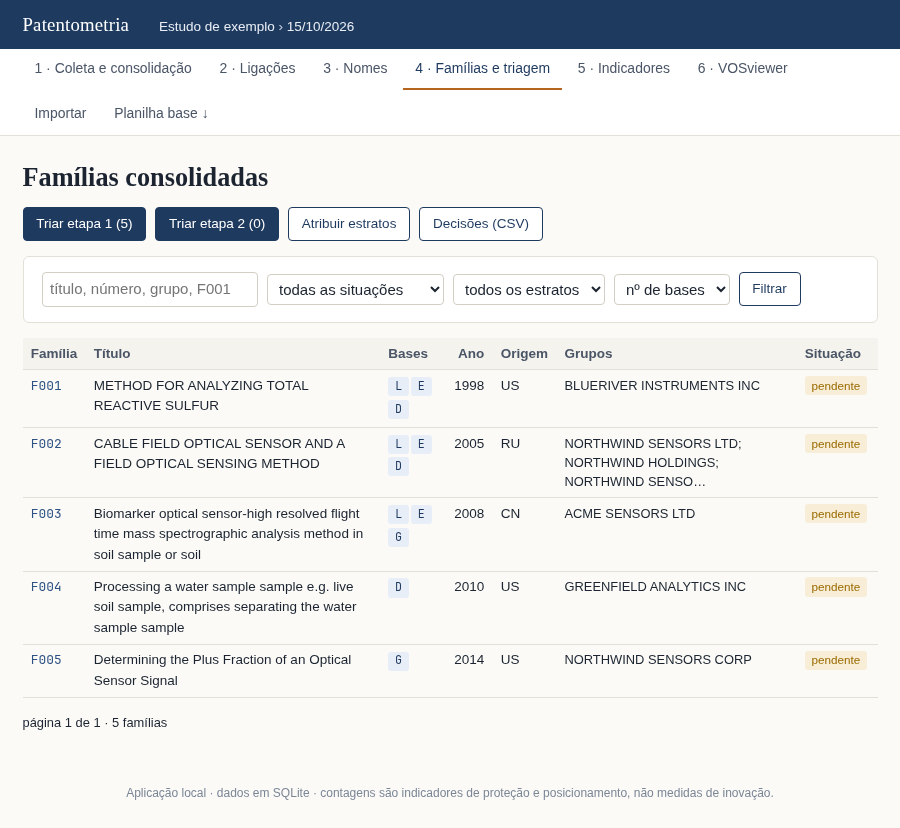
\includegraphics[width=0.82\linewidth]{img/06_familias.png}
\caption{Lista de famílias da rodada, com chave, título, número de bases, documentos e situação na
triagem.}
\label{fig:familias}
\end{figure}

\begin{figure}[H]
\centering
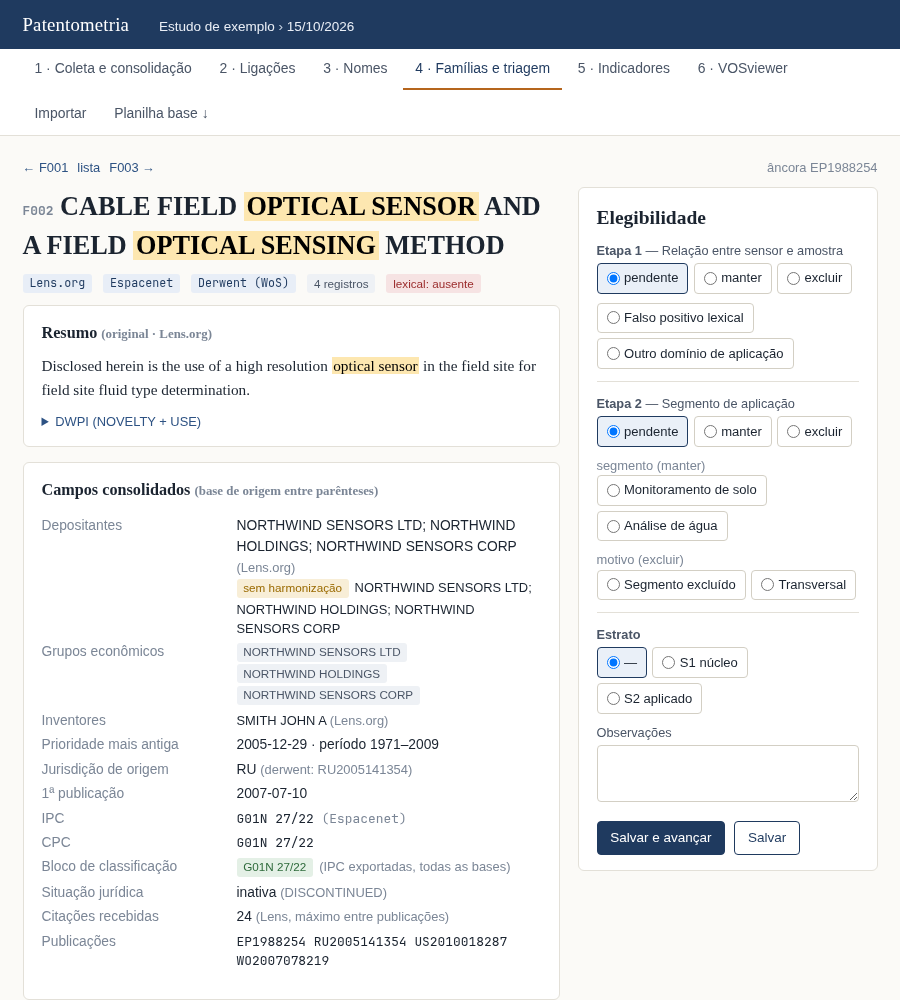
\includegraphics[width=0.75\linewidth]{img/07_familia_topo.png}
\caption{Ficha da família F002: dados consolidados, título e resumo com destaques, e os registros
originais de cada base.}
\label{fig:familia}
\end{figure}

\subsection*{O que fazer}
\begin{enumerate}
\item Abra \textbf{Famílias} e ordene pela coluna que interessa (bases, documentos, chave).
\item Clique em uma família para abrir a ficha.
\item Confira os dados consolidados e abra a lista de registros originais.
\item Se houver divergência entre bases, registre na observação da triagem.
\end{enumerate}

\subsection*{Como interpretar}
A chave (\campo{F001}, \campo{F002}) é interna e serve para navegar; não é um identificador de patente.
O \textbf{número de bases} mostra a cobertura; o número de \textbf{documentos} mostra quantos registros
foram agrupados naquela família.

Na ficha, os campos consolidados vêm de regras de precedência: o título original da família, a
prioridade mais antiga, o conjunto de depositantes e as classificações. Quando as bases divergem, a
aplicação escolhe um valor e mantém os originais visíveis --- a divergência é informação, não erro a
ser apagado.

\begin{nota}[Registro original é a fonte]
Sempre que um número parecer estranho, volte ao registro original. Título traduzido, resumo truncado
e prioridade ausente são as três causas mais comuns de discordância entre bases.
\end{nota}

\begin{alerta}[Erro comum]
Usar a chave interna em uma citação. Em texto, cite o número de publicação ou a prioridade; a chave
muda a cada rodada.
\end{alerta}

\subsection*{Checkpoint}
\marcador\; Você consegue explicar, para uma família qualquer, quantos documentos ela tem, de quais bases
e qual é a prioridade mais antiga.
